\documentclass{article}
\usepackage[utf8]{inputenc}
\usepackage{listings}
\usepackage{hyperref}
\usepackage{titlesec}
\usepackage{graphicx}
\usepackage{subcaption}

\title{Probabilistic Programming}
\author{Gillis Hermans, Sven Thijssen}
\date{March 2019}

\begin{document}

\maketitle
\tableofcontents

\newpage

\section{Probabilistic Inference Using Weighted Model Counting}

\subsection{PGM to CNF}

The Bayesian network with full CPTs can be rewritten as noisy-ORs. We therefore assume the following \cite{noisyor}:
\begin{itemize}
    \item All possible causes $X_i$ for an event $Y$ are listed
    \item The negated clauses $\neg X_i$ do not have an influence on $Y$
    \item Independent failure probability $q_i$ for each cause alone
\end{itemize}

We can observe that if all diseases are False, the occurrence of a symptom is not $0$ but rather $0.1$ for each of the symptoms. We therefore introduce a leaky node with a probability $l = P(P(Y \mid \bar{X_i}, \forall i = 1..n)$.
Using this leaky probability, we can compute the leaky noisy OR as follows:
$$P(Y \mid X_i) = 1-(1-l) \times \prod_{X_i \in X_T}\frac{1-p_i}{1-l}$$\\
and
$$P(\bar{Y} \mid X_i) = (1-l) \times \prod_{X_i \in X_T}\frac{1-p_i}{1-l}$$\\

For the Bayesian network, we obtain the probabilities given in Table \ref{tab:leakynoisyor}. We also know the following:
$P(X_I) = 0.05$, 
$P(\bar{X_I}) = 1 - 0.05 = 0.95$, 
$P(X_O) = 0.01$, 
$P(\bar{X_O}) = 1 - 0.01 = 0.99$, 
$P(X_R) = 0.0001$, 
$P(\bar{X_R}) = 1 - 0.0001 = 0.9999$.\footnote{We indicate both diseases and symptoms by their first letter.}

\begin{table}[h]
\centering
\begin{tabular}{l l l l | l | l | l | l}
	\hline
	$X_I$	&	$X_O$	&	$X_R$	&	$L$		&	$P(Y_T)$		&	$P(Y_S)$		&	$P(Y_N)$\\
	\hline
	F		&	F		&	F		&	T		&	0.10			&	0.10			&	0.10\\
	F		&	F		&	T		&	T		&	0.73			&	0.9910		&	0.55\\
	F		&	T		&	F		&	T		&	0.10			&	0.9910		&	0.10\\
	T		&	F		&	F		&	T		&	0.64			&	0.19			&	0.2350\\
	\hline
\end{tabular}
\caption{Leaky noisy-OR}
\label{tab:leakynoisyor}
\end{table}

For the first part of the assignment, we have written a program\footnote{Source code on GitHub: \href{https://github.com/sventhijssen/pgmtocnf}{https://github.com/sventhijssen/pgmtocnf}} to compute both \texttt{ENC1} and \texttt{ENC2}, based on a given probabilistic graphical model. We created a graph structure which represented the conditional probability table of the Bayesian network. For the noisy-OR, we adapted our code with minimal changes: we created a new type of graph (\texttt{NoisyGraph}) with a leaky probability value. See \hyperref[appendix]{Appendix} for the CNF and associated weights.

\newpage
 
\subsection{SRL to CNF}
\subsubsection{CNF and associated weights}
\underline{\textbf{Write the encoding for the ProbLog program as CNF and associated weights.}}
\\
For this task we followed the approach of \cite{Fierens} which is split into three steps. Ground the program so that it only contains the necessary part needed for the given evidence and query. Convert the following ground rules to CNF and finally define a weight function for all atoms. \footnote{Source code on GitHub: \href{https://github.com/gillishermans/probabilisticprogramming_part1.2-3}{https://github.com/gillishermans/probabilisticprogramming\_part1.2-3}}
\\\\
\underline{\textbf{Grounding}}
\\
If there are positive and negative rules of f these are changed into a $f\_p$ and a $f\_n$ which are then combined to $f :- f\_p,  \neg f\_n.$. All atoms and rules are ground according to the dependancy set of the evidence E and the query Q. Rules that have no relevance to the evidence and query will be removed from the program. 
\\\\
\textbf{The inititial problog program:}
\\
$increaseOsteoblasts :- calcium.\\
0.5::\neg increaseOsteoblasts :- calcium, bispho.\\
reduceOsteoclasts :- bispho.\\
1.0::\neg reduceOsteoclasts :- calcium , bispho.\\
osteoprosis :- initialOsteoprosis.\\
0.85::\neg osteoprosis :- reduceOsteoclasts.   \% Bisphosphonates\\
0.15::\neg osteoprosis :- increaseOsteoblasts. \% Calcium\\
\% Prior probabilities\\
0.5::calcium. 0.5::bispho. 0.5::initialOsteoprosis.\\
\% Query probability of effect\\
evidence(initialOsteoprosis, true).\\
evidence(calcium, true).\\
evidence(bispho, false).\\
query(osteoprosis).$\\
\\
\textbf{The ground problog program:}
\\
$
increaseOsteoblasts :- increaseOsteoblasts_p, \neg increaseOsteoblasts_n.\\
increaseOsteoblasts_p :- calcium.\\
0.5::increaseOsteoblasts_n :- calcium, bispho.\\
reduceOsteoclasts :- reduceOsteoclasts_p, \neg reduceOsteoclasts_n.\\
reduceOsteoclasts_p :- bispho.\\
1.0::reduceOsteoclasts_n :- calcium, bispho.\\
osteoprosis_p :- initialOsteoprosis.\\
0.85::osteoprosis_n :- reduceOsteoclasts.\\
0.15::osteoprosis_n :- increaseOsteoblasts.\\
osteoprosis :- osteoprosis_p, \neg osteoprosis_n.\\
0.5::calcium. 0.5::bispho. 0.5::initialOsteoprosis.\\
evidence(initialOsteoprosis, true).\\
evidence(calcium, true).\\
evidence(bispho, false).\\
query(osteoprosis).$\\
\underline{\textbf{CNF}}
\\
Next the ground program is converted into a CNF. Cyclical rules are ignored as they are removed from the grounded program before converting into CNF form (even though there are no cyclical rules in this specific example). The Clark's completion of the rules is made to transform the problog rules into first-order logic. This can then simply be rewritten to a CNF form found in de dimacs file provided.
\\\\
\textbf{The clark's completion:}
\\
$
increaseOsteoblasts \leftrightarrow increaseOsteoblasts_p \land \neg increaseOsteoblasts_n\\
increaseOsteoblasts_p \leftrightarrow calcium\\
increaseOsteoblasts_n \leftrightarrow calcium \land bispho.\\
reduceOsteoclasts \leftrightarrow reduceOsteoclasts_p \land \neg reduceOsteoclasts_n.\\
reduceOsteoclasts_p \leftrightarrow bispho.\\
reduceOsteoclasts_n \leftrightarrow calcium \land bispho.\\
osteoprosis_p \leftrightarrow initialOsteoprosis.\\
osteoprosis_p \leftrightarrow initialOsteoprosis.\\
osteoprosis_n \leftrightarrow reduceOsteoclasts.\\
osteoprosis_n \leftrightarrow increaseOsteoblasts.\\
osteoprosis \leftrightarrow osteoprosis_p \land \neg osteoprosis_n.\\
calcium
\neg bispho
initialOsteoprosis
$
\\\\
\underline{\textbf{Weights}}
\\
Finally the weights of each probabilistic fact $p::f$ will be assigned $p$ as a weight and $\neg f$ will be assigned $1-p$. Literals not occuring in a probabilistic fact will get weight 1. The probabilistic rules are first rewritten to both a deterministic rule and a probabilistic fact to facilitate assigning the probabilistic facts a weight. $p :: f :- g.$ becomes $p :: f\_fact.$ $f :- g, f\_fact.$
\\\\
\textbf{The ground problog program rewritten:}
\\
$
increaseOsteoblasts :- increaseOsteoblasts_p, \neg increaseOsteoblasts_n.\\
increaseOsteoblasts_p :- calcium.\\
0.5::increase_{n_fact}.\\
increaseOsteoblasts_n :- calcium, bispho, increase_{n_fact}.\\
reduceOsteoclasts :- reduceOsteoclasts_p, \neg reduceOsteoclasts_n.\\
reduceOsteoclasts_p :- bispho.\\
1.0::reduce_{n_fact}.\\
reduceOsteoclasts_n :- calcium, bispho, reduce_{n_fact}.\\
osteoprosis_p :- initialOsteoprosis.\\
0.85::osteoprosis_reduce_fact.\\
osteoprosis_n :- reduceOsteoclasts, osteoprosis_reduce_fact.\\
0.15::osteoprosis_increase_fact.\\
osteoprosis_n :- increaseOsteoblasts , osteoprosis_increase_fact.\\
osteoprosis :- osteoprosis_p, \neg osteoprosis_n.\\
0.5::calcium. 0.5::bispho. 0.5::initialOsteoprosis.\\
evidence(initialOsteoprosis, true).\\
evidence(calcium, true).\\
evidence(bispho, false).\\
query(osteoprosis).$\\
\\\\
\textbf{The weights (not occuring in this list have weight 1):}
\\
$
calcium \rightarrow 0.5\\
\neg calcium \rightarrow 0.5\\
bispho \rightarrow 0.5\\
\neg bispho \rightarrow 0.5\\
initialOsteoprosis \rightarrow 0.5\\
\neg initialOsteoprosis \rightarrow 0.5\\
increase_{n_fact} \rightarrow 0.5\\
\neg increase_{n_fact} \rightarrow 0.5\\
reduce_{n_fact} \rightarrow 1.0\\
\neg reduce_{n_fact} \rightarrow 0.0\\
osteoprosis_{reduce_fact} \rightarrow 0.85\\
\neg osteoprosis_{reduce_fact} \rightarrow 0.15\\
osteoprosis_{increase_fact} \rightarrow 0.15\\
\neg osteoprosis_{increase_fact} \rightarrow 0.85\\
$

\newpage

\subsection{Weighted Model Counting}

\subsubsection{Weighted model counting}
In Table \ref{tab:wmc_pysdd_cachet}, we observe that the weighted model count for the different encodings using  \textit{PySDD} holds a value of approximately $1$. This is what we would expect: the weighted model count of the theory $\Delta$ is equivalent with summing all probabilities in the joint distribution. This WMC could be interpreted as the probability that any model is chosen, which says nothing about the model. 
$$WMC(\Delta) = \sum_{\omega \models \Delta} W(\omega)$$
where
$$W(\omega) = \prod_{\omega \models l}W(l)$$
with $W(\omega)$ the weight assigned to each literal $l$.\cite{chavira}\\
For \textit{Cachet} we could not obtain a probability of 1 nor any solutions when adding weights to the CNF file. However, when leaving the weights out, we obtain the same model count (64) as with \textit{PySDD}.
\footnote{We were unable to test any other Exact Model Counter due to compilation errors. Also some lines of code had to be adjusted to make \textit{Cachet} compile.}
\begin{table}[h]
\centering
\begin{tabular}{l | l l}
					&	PySDD	&		Cachet	\\\hline
	Full CPT ENC1	&	1.0000000000000002		&		?		\\
	Noisy OR ENC1	&	0.9998172061924634		&		?		\\
	Full CPT ENC2	&	1.0 &	?	\\
	Noisy OR ENC2	&	1.0		&		?		\\
\end{tabular}
\caption{WMC for \textit{PySDD} and \textit{Cachet} using \texttt{ENC1} and \texttt{ENC2}}
\label{tab:wmc_pysdd_cachet}
\end{table}

For \textit{PySDD} and \textit{Cachet}, we executed the following commands respectively:
\begin{itemize}
	\item[] \texttt{\$ python3 pysdd-cli.py -c [enc1|enc2]\_[full|noisy]\_pysdd.cnf}
	\item[] \texttt{\$ ./cachet [enc1|enc2]\_[full|noisy]\_cachet.cnf}
\end{itemize}

\newpage

\subsubsection{Smallest circuit}
``An SDD normalized for a vtree $v$ is a Boolean circuit defined as follows. If $v$ is a leaf node labeled with variable $X$, then the SDD is either $X$, $\neg X$, $\bot$ or an or-gate with inputs $X$ and $\neg X$ [\dots]''\cite{shen}.\\
From the output, we get the SDD size, which is the size of the smallest circuit since the model is already minimized.
For the different encodings, we vary the initial vtree type (flag \texttt{-t}) and the clauses for vtree search (flag \texttt{-r}).


\begin{figure}[h]
  \centering
  \begin{subfigure}[b]{0.4\linewidth}
    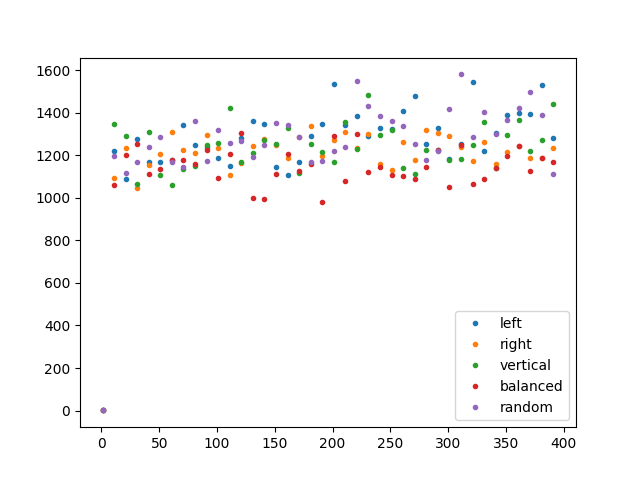
\includegraphics[width=\linewidth]{images/standard_enc1_full.png}
    \caption{Circuit size for Bayesian net as full CPT with \texttt{ENC1} for varying vtree type and number of clauses for vtree search}
  \end{subfigure}
    \begin{subfigure}[b]{0.4\linewidth}
    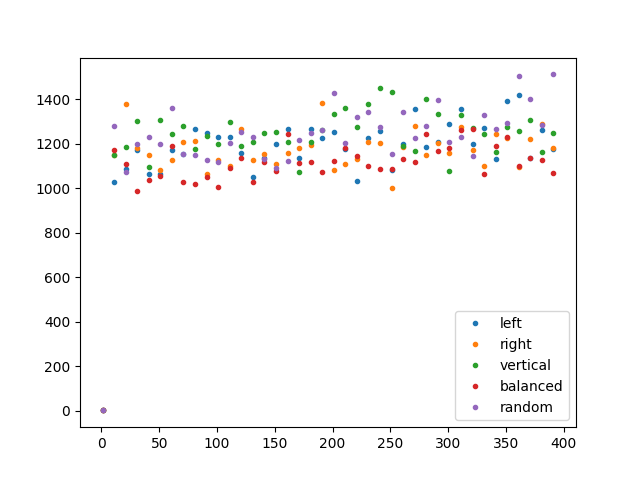
\includegraphics[width=\linewidth]{images/standard_enc1_noisy.png}
    \caption{Circuit size for Bayesian net as noisy-OR with \texttt{ENC1} for varying vtree type and number of clauses for vtree search}
  \end{subfigure}
  \begin{subfigure}[b]{0.4\linewidth}
    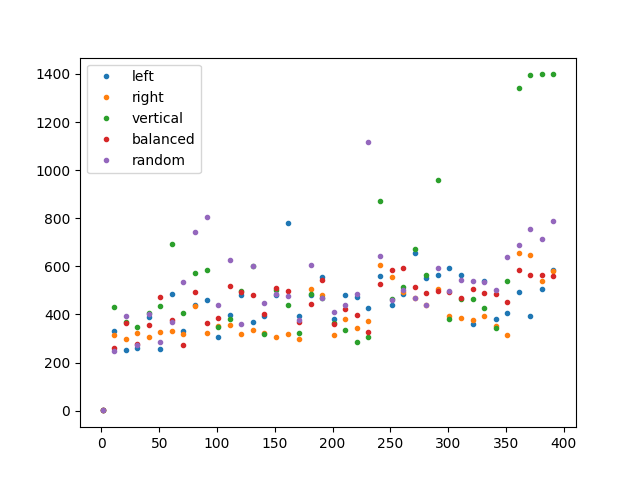
\includegraphics[width=\linewidth]{images/standard_enc2_full.png}
    \caption{Circuit size for Bayesian net as full CPT with \texttt{ENC2} for varying vtree type and number of clauses for vtree search}
  \end{subfigure}
    \begin{subfigure}[b]{0.4\linewidth}
    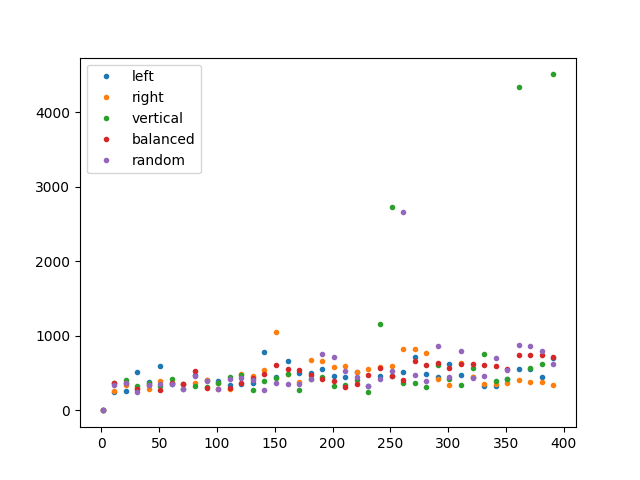
\includegraphics[width=\linewidth]{images/standard_enc2_noisy.png}
    \caption{Circuit size for Bayesian net as noisy-OR with \texttt{ENC2} for varying vtree type and number of clauses for vtree search}
  \end{subfigure}
  \label{fig:circuits}
\end{figure}

We observe that the circuit size is overall smaller for balanced vtrees and overall greater for random vtrees. Circuit sizes for left and right  vtrees usually lie between these circuit values. Vertical vtrees seem to be prone to outliers.

For this task, we executed the following command\footnote{Source code on GitHub: \href{https://github.com/sventhijssen/pysdd}{https://github.com/sventhijssen/pysdd}}
\begin{itemize}
	\item[] \texttt{\$ python3 hyperparam-cli.py}
\end{itemize}

\newpage

\subsubsection{Computational requirements}
To create an overview of the runtime and memory usage of the python process, we used \textit{Pympler}. In Table \ref{tab:memory_runtime}, we observe that the memory usage for all representations is approximately the same. The runtime, however, for \texttt{ENC2} is much lower than for \texttt{ENC1}.

\begin{table}[h]
\centering
\begin{tabular}{l | l l}
					&	Memory (kB)	&	Runtime (s)	\\\hline
	Full CPT ENC1	&	8542.77		&	0.45			\\
	Noisy OR ENC1	&	8543.17		&	0.62			\\
	Full CPT ENC2	&	8543.56		&	0.13			\\
	Noisy OR ENC2	&	8543.98		&	0.15			\\
\end{tabular}
\caption{Computational requirements (memory and runtime) for \texttt{ENC1} and \texttt{ENC2}}
\label{tab:memory_runtime}
\end{table}

For this task, we executed the following command\footnote{Source code on GitHub: \href{https://github.com/sventhijssen/pysdd}{https://github.com/sventhijssen/pysdd}}:
\begin{itemize}
	\item[] \texttt{\$ python3 compreq-cli.py}
\end{itemize}

\subsubsection{Probabilities}
To compute the probability $P(S \mid I=\top, O = \top, R = \top)$, we add evidence to the theory $\Delta$. As mentioned by Chavria and Darwiche \cite{chavira}, there are two ways to incorporate this evidence:
\begin{enumerate}
	\item the weight associated with each indicator $\lambda_x$, whose subscript contradicts the evidence from 1 to 0.
	\item the rows that contradicts the evidence are removed from the theory being counted.
\end{enumerate}

To obtain these results, we have chosen to use the first approach. We have adapted our script which generates the \textit{PySDD} CNF file such that the $\lambda_x$ indicator variables which contradict the evidence are set to 0. However, when using this technique, we obtained results which did not match our expectations. We would expect the probability to be $99.99\%$ (see Figure \ref{fig:task_1_3_4}) but obtained a WMC of 0, which would be incorrect. We then made a script to load the \textit{PySDD} CNF file and set the weights of the literals manually. When doing this, the probabilities of the literals are $nan$.

\subsubsection{Theoretical differences}
A distinction is made between bottom-up compilers and top-down compilers. \textit{SDD} and thus \textit{PySDD} which builds upon \textit{SDD} is a bottom-up compiler. \textit{miniC2D} is a top-down compiler. Bottom-up compilers construct a full knowledge base by merging smaller chunks (e.g. clauses of a CNF) of a knowledge base by means of an \texttt{apply} operation.\cite{topdown} The \texttt{apply} operation either conjoins or disjoins two SDDs. \cite{bottomup} The top-down compilers starts from a full knowledge base and recursively compiles fragments and then merges them to make a compilation of a full knowledge base.\cite{topdown}\footnote{We were unable to find whether \textit{Cachet} is a top-down or bottom-up compiler. We do know \textit{Cachet} builds further upon \textit{zChaff} and uses the \textit{DPLL} algorithm. We assume it is bottom-up since it learns from clauses and iteratively builds up the knowledge base.}

\newpage

\begin{figure}[h]
	\centering
	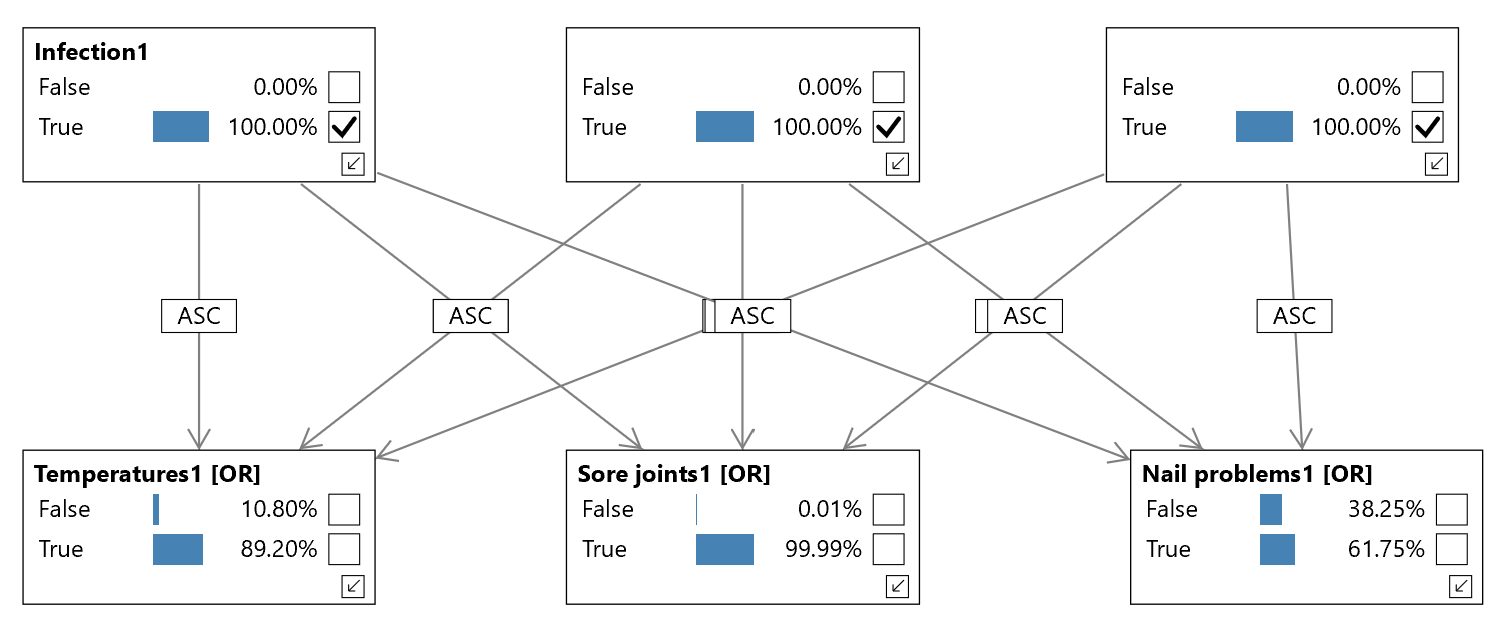
\includegraphics[width=\linewidth]{images/task_1_3_4.png}
	\caption{Probability}
	\label{fig:task_1_3_4}
\end{figure}

\section{Lifted Inference}
\subsection{Lifted inference rules}
In order to compute $P(sorejoints|infection=T,osteo=T,rheuma=T)$ we use the lifted inference rules to transform this query. First of all the query is transformed into a FOL statement:
\begin{center}
    $Q = \exists$ x i(x) $\land$ o(x) $\land$ r(x) $\land$ sj(x)
\end{center}
To compute $P(Q)$ the following lifted inference steps are taken:
\begin{center}
    $\exists$-rule: $P(Q) = 1 - \prod_{c \in Domain} (1-P(i(C)\land o(C) \land r(C) \land sj(C))) $\\
    $\land$-rule: $P(Q) = 1 - \prod_{c \in Domain} (1-P(i(C))P(o(C))P(r(C))P(sj(C)))) $\\
\end{center}
The obtained probabilities can simply be looked up in the probabilistic database.

\subsection{Alternative encodings}
We have not found a solution to this task.


\section{Parameter Learning}
\subsection{Generate interpretations}
We have generated the 4 following interpretations while dropping observations with probability 30\% using the problog sample function:
\begin{itemize}
    \item\{osteoprosis: True, calcium: True, bispho: False\}
    \item\{osteoprosis: False, calcium: False\}
    \item\{osteoprosis: False, bispho: False, initialOsteoprosis: False\}
    \item\{osteoprosis: True, bispho: False initialOsteoprosis: True\}
\end{itemize}
\subsection{Estimate parameters}
In order to estimate the parameters $p_{n}$ for every fact in the problog program we query each of those facts for a number of interpretations $m$ \footnote{Source code on GitHub: \href{https://github.com/gillishermans/probabilisticprogramming_part1.2-3}{https://github.com/gillishermans/probabilisticprogramming\_part1.2-3}}. These interpretations are generated as in the previous section.\\\\
For every interpretation we start from the model problog program without evidence and add the observations in the interpretation as evidence. However any observations about the current fact are removed from the evidence. Otherwise the evaluation would give either 0.0 (if there was an observation that the fact was false) or 1.0(true). This would skew the estimated parameter. Next we add the fact as a query and evaluate with problog. These evaluations are summed and divided by the number of interpretations $m$. This is the new learned parameter $p_{n}$:
\begin{center}
    $p_{n} = \frac{1}{M} \sum_{m=1}^M P(f_{n}|I_{m}) $\\
    where $I_{m}$ is the $m$'th interpretation.
\end{center}
The learned parameters are:
\begin{table}[h!]
    \begin{center}
    \begin{tabular}{|l|l|l|l|l|}
    \hline
                    & actual   & 100        & 1000      & 10000     \\ \hline
    bispho              & 0.5      & 0.4905147  & 0.5027595 & 0.4993673 \\ \hline
    calcium             & 0.5      & 0.51874435 & 0.4977120 & 0.5027093 \\ \hline
    initialOsteoprosis  & 0.5      & 0.5504062  & 0.4933254 & 0.5020656 \\ \hline
    osteoprosis         & 0.365625 & 0.4188750  & 0.3704031 & 0.3642547 \\ \hline
    reduceOsteoclasts   & 0.25     & 0.1793807  & 0.2527558 & 0.2506215 \\ \hline
    increaseOsteoblasts & 0.375    & 0.4437956  & 0.3806887 & 0.3742494          \\ \hline
    \end{tabular}
    \caption{The learned parameters.}
    \label{tab:param}
    \end{center}
\end{table}
\subsection{Explain observations}
As expected bispho, calcium and initialOsteoprosis are estimated around 0.5. This is the probability given to them in the problog program itself. The rest of the estimates are accurate as well. The actual probabilities can be found by evaluating the problog program without evidence and with the fact as a query. It is also possible to manually show that for example the probability of reduceOsteoclasts is 25\%. The  following problog rules clearly define the probabilities given in table \ref{tab:reduce}.
\begin{center}
    $reduceOsteoclasts :- bispho.$\\
    $1.0::\neg reduceOsteoclasts :- calcium , bispho.$\\
    $0.5::calcium. 0.5::bispho.$
\end{center}
\begin{table}[h!]
    \begin{center}
    \begin{tabular}{|ll|l|l|}
    \hline
    bispho       & calcium       & $\sim$reduceOsteoclasts & 0.25 \\
    $\sim$bispho & calcium       & $\sim$reduceOsteoclasts & 0.25 \\
    bispho       & $\sim$calcium & reduceOsteoclasts       & 0.25 \\
    $\sim$bispho & $\sim$calcium & $\sim$reduceOsteoclasts &     0.25 \\ \hline
    \end{tabular}
    \caption{ReduceOsteoclasts table.}
    \label{tab:reduce}
    \end{center}
\end{table}

Of course with a higher number of interpretations a more accurate estimate will be achieved as can be seen in the table of the learned paramaters. However 10000 iterations does not seem to have an advantage over 1000 iterations. The runs will take 10 times longer and are not significantly more accurate. 

\subsection{Learn positive or negative influence}
A possibility is to compare two different estimates (using the same or similar technique to the previous question). One where part of every interpretation has an observation that the investigated variable is true, and one where it is false.
\begin{center}
    $P(f_{n}|I_{m} \land investigated=T)$\\
    $P(f_{n}|I_{m} \land investigated=F)$
\end{center}
These estimates can be compared to see if in general the investigated variable has a positive or negative effect on fact $f_{n}$.

\newpage


\section*{Repositories}
\begin{itemize}
	\item \href{https://github.com/sventhijssen/pgmtocnf}{https://github.com/sventhijssen/pgmtocnf}
	\item \href{https://github.com/gillishermans/probabilisticprogramming_part1.2-3}{https://github.com/gillishermans/probabilisticprogramming\_part1.2-3}
	\item \href{https://github.com/sventhijssen/pysdd}{https://github.com/sventhijssen/pysdd}
\end{itemize}

\bibliography{references}
\bibliographystyle{ieeetr}

\newpage

\section*{Appendix}
\label{appendix}
\subsubsection*{Full CPTs with ENC1}
\paragraph{Variables}\mbox{}\\
\input{../out/enc1_full_enc.tex}
\newpage
\paragraph{Weights}\mbox{}\\
\input{../out/enc1_full_weights.tex}

\newpage

\subsubsection*{Noisy-ORs with ENC1}
\paragraph{Variables}\mbox{}\\
\input{../out/enc1_noisy_enc.tex}
\newpage
\paragraph{Weights}\mbox{}\\
\input{../out/enc1_noisy_weights.tex}

\newpage

\subsubsection*{Full CPTs with ENC2}
\paragraph{Variables}\mbox{}\\
\input{../out/enc2_full_enc.tex}
\newpage
\paragraph{Weights}\mbox{}\\
\input{../out/enc2_full_weights.tex}

\newpage

\subsubsection*{Noisy-ORs with ENC2}
\paragraph{Variables}\mbox{}\\
\input{../out/enc2_noisy_enc.tex}
\newpage
\paragraph{Weights}\mbox{}\\
\input{../out/enc2_noisy_weights.tex}

\end{document}
